% ============================================================
% BLOC 2: ESPECIFICACIÓ  (diapositives 5–7)
% BLOC 3: DISSENY I ARQUITECTURA  (diapositives 8–12)
% ============================================================

% ---  DIAPOSITIVA 5 — Els Actors del Sistema  ---
\begin{frame}{Els Actors del Sistema}
  \vspace{0.2em}
  \begin{columns}[T]
    \begin{column}{0.3\textwidth}
      \begin{block}{Administrador}
        \begin{itemize}
          \item[\small$\bullet$] Configuració completa.
          \item[\small$\bullet$] Gestió d'usuaris.
          \item[\small$\bullet$] Actualitzacions de firmware.
        \end{itemize}
      \end{block}
    \end{column}

    \begin{column}{0.3\textwidth}
      \begin{block}{Operador}
        \begin{itemize}
          \item[\small$\bullet$] Vídeo en directe.
          \item[\small$\bullet$] Gravacions i timeline.
          \item[\small$\bullet$] Gestió d'alarmes.
        \end{itemize}
      \end{block}
    \end{column}

    \begin{column}{0.3\textwidth}
      \begin{block}{Sistema NVR}
        \begin{itemize}
          \item[\small$\bullet$] Emet esdeveniments push.
          \item[\small$\bullet$] Dicta l'esquema JSON.
          \item[\small$\bullet$] Gestiona els \textit{config locks}.
        \end{itemize}
      \end{block}
    \end{column}
  \end{columns}

  \vspace{0.8em}
  \begin{center}
    \textbf{6 casos d'ús principals:} Autenticació $\cdot$ Vídeo directe $\cdot$ Gravacions $\cdot$ Alarmes $\cdot$ Configuració dinàmica $\cdot$ Administració
  \end{center}

  \note{
    L'anàlisi d'actors va revelar tres rols principals. L'Administrador té accés total: pot configurar el sistema, gestionar usuaris i actualitzar el firmware. L'Operador és el vigilant del dia a dia: veu les càmeres, revisa gravacions i gestiona alarmes. I el Sistema NVR actua com a tercer actor: és qui dicta les regles del joc mitjançant l'esquema JSON, qui emet els esdeveniments d'alarma, i qui gestiona els mecanismes de control d'accés a la configuració.

    A partir d'aquests actors vam derivar 6 casos d'ús principals que cobreixen tot el cicle de vida de la vigilància: autenticació segura, visualització de vídeo en directe, cerca de gravacions en una línia de temps, gestió d'alarmes, configuració dinàmica basada en esquema, i administració del sistema.
  }
\end{frame}

% ---  DIAPOSITIVA 6 — Requisits Crítics: Rendiment  ---
\begin{frame}{Requisits Crítics: Rendiment i Vídeo}
  \begin{columns}[T]
    \begin{column}{0.48\textwidth}
      \begin{alertblock}{RNF-01: Latència de vídeo}
        \begin{itemize}
          \item Objectiu: \textbf{$<$ 300 ms} de latència mitjana.
          \item P95: $<$ 350 ms.
          \item Motiu: sales de monitorització activa.
        \end{itemize}
      \end{alertblock}
    \end{column}

    \begin{column}{0.48\textwidth}
      \begin{alertblock}{RNF-03: Eficiència de CPU}
        \begin{itemize}
          \item Zero \textit{polling} HTTP.
          \item Actualitzacions granulars (\textit{Signals}).
          \item NGINX $\leq$ 5\% overhead addicional.
        \end{itemize}
      \end{alertblock}
    \end{column}
  \end{columns}

  \vspace{0.6em}
  \begin{columns}[T]
    \begin{column}{0.48\textwidth}
      \begin{block}{RNF-02: Fallback automàtic}
        Si UDP bloquejat: commuta a HLS en $\leq$ \textbf{5 segons}.
      \end{block}
    \end{column}

    \begin{column}{0.48\textwidth}
      \begin{block}{RNF-04: WebSocket resilient}
        Reconexió automàtica en $\leq$ \textbf{30 segons} (backoff exponencial).
      \end{block}
    \end{column}
  \end{columns}

  \note{
    Traduïm l'objectiu de negoci en requisits mesurables. El més crític és el de latència: en una sala de control de seguretat, si el vídeo va amb 2 segons de retard, una intrusió pot passar desapercebuda. Per això vam fixar 300 ms com a límit dur per al temps real.

    Igualment important és l'eficiència de CPU. L'NVR té una CPU ARM limitada. Si l'aplicació web consumeix massa processador al client, l'operador de vigilància veurà el seu PC aturats. Per això vam descartar qualsevol arquitectura basada en polling i vam apostar per actualitzacions push i reactivitat granular.

    I per cobrir les xarxes corporatives que bloquejen UDP ---molt habituals en entorns industrials--- vam especificar un fallback automàtic a HLS en menys de 5 segons.
  }
\end{frame}

% ---  DIAPOSITIVA 7 — Requisits Crítics: Seguretat  ---
\begin{frame}{Requisits Crítics: Seguretat i Privadesa}
  \begin{columns}[T]
    \begin{column}{0.48\textwidth}
      \textbf{Seguretat (OWASP Top 10)}
      \begin{itemize}
        \item Sense \textit{LocalStorage} per a credencials.
        \item Cookies \textbf{HttpOnly + Secure + SameSite}.
        \item Xifratge \textbf{TLS 1.2/1.3} i \textbf{WSS}.
        \item Immunitat XSS i CSRF per disseny.
      \end{itemize}
    \end{column}

    \begin{column}{0.48\textwidth}
      \textbf{Privadesa (RGPD / LOPDGDD)}
      \begin{itemize}
        \item \textbf{Privacy by Design}: dades sensibles només a RAM.
        \item Zero persistència al recarregar la pàgina.
        \item UNE-EN 62676: retenció 24h--30 dies.
        \item Sense emmagatzematge biometria.
      \end{itemize}
    \end{column}
  \end{columns}

  \vspace{0.6em}
  \begin{center}
    \begin{block}{}
      \centering La seguretat no és una capa afegida: és una \textbf{restricció de disseny} des del primer dia.
    \end{block}
  \end{center}

  \note{
    La seguretat en un sistema de videovigilància professional no és opcional. Estem tractant amb imatges de persones, dades sensibles, i infraestructura crítica. Per això vam imposar-nos el compliment de l'OWASP Top 10 com a criteri d'acceptació.

    La decisió més important va ser no emmagatzemar mai credencials al LocalStorage del navegador, que és accessible per qualsevol script de la pàgina. En el seu lloc, la sessió es gestiona amb cookies HttpOnly, que el navegador envia automàticament però que cap JavaScript pot llegir. Això elimina d'arrel els atacs de robatori de sessió per XSS.

    I per complir amb el RGPD, vam implementar el principi de Privacy by Design: si l'operador recarrega la pàgina, la sessió expira i les dades sensibles desapareixen de la memòria. Zero persistència per defecte.
  }
\end{frame}

% ---  DIAPOSITIVA 8 — Arquitectura Global  ---
\begin{frame}{Arquitectura Global del Sistema}
  \vspace{0.2em}
  \begin{columns}[T]
    \begin{column}{0.52\textwidth}
      \begin{center}
        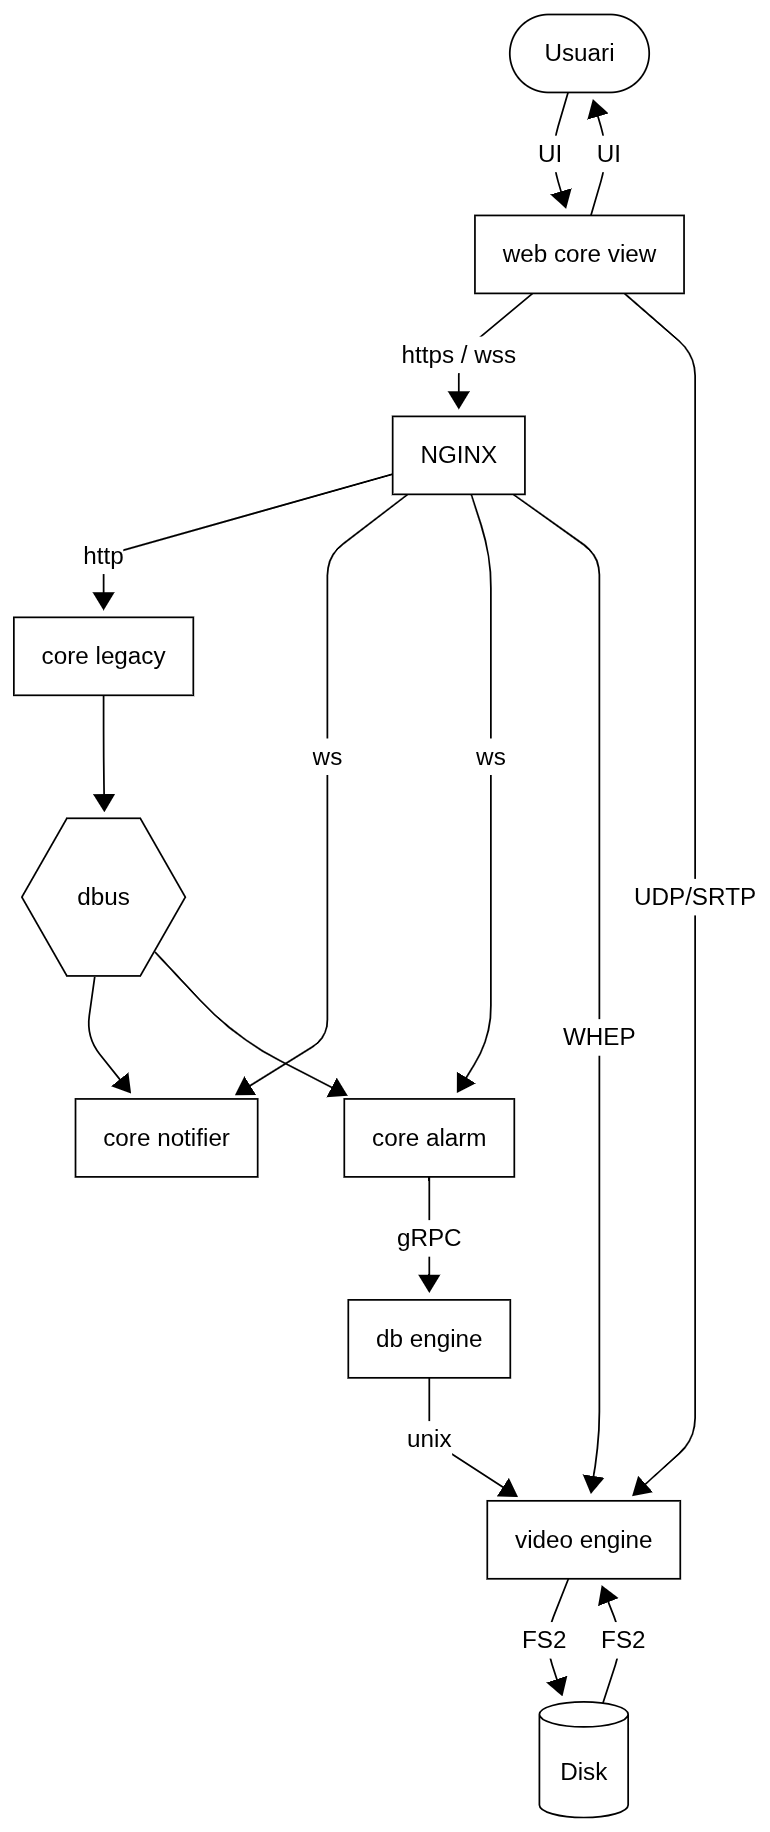
\includegraphics[width=\textwidth,keepaspectratio]{../figures/diagrames/arquitectura_serveis.png}
      \end{center}
    \end{column}
    \begin{column}{0.44\textwidth}
      \begin{itemize}
        \item \textbf{SPA:} Angular renderitza al navegador --- allibera la CPU del gravador.
        \item \textbf{Microserveis C++:} cada procés gestiona un domini aïllat.
        \item \textbf{NGINX:} únic punt d'entrada, gestiona seguretat i routing.
      \end{itemize}
    \end{column}
  \end{columns}

  \note{
    El disseny arquitectònic respon directament als requisits de recursos limitats. En comptes d'un servidor monolític que tot ho processa, tenim una separació clara de responsabilitats.

    L'Angular és una Single-Page Application: es descarrega una vegada i s'executa completament al navegador del client. Això significa que el processament de la interfície, els càlculs de l'estat, les animacions, tot recau al PC de l'operador i no en la CPU del gravador.

    Al backend, cada responsabilitat és un procés C++ independent: un per a la configuració i autenticació, un per al motor de vídeo, un per a les alarmes. Aquesta separació permet que si el motor de vídeo falla, la configuració continuï funcionant.

    Entre els dos mons, NGINX actua com a porter: tota petició del navegador ha de passar per ell. Ell decideix a quin microservei la reenviar, gestiona el TLS i imposa les regles de seguretat.
  }
\end{frame}

% ---  DIAPOSITIVA 9 — Microserveis al Dispositiu  ---
\begin{frame}{Els Microserveis al Dispositiu}
  \vspace{0.2em}
  \begin{columns}[T]
    \begin{column}{0.48\textwidth}
      \begin{block}{Capa de comunicació}
        \begin{itemize}
          \item \texttt{la-core-legacy} --- Config API, Auth.
          \item \texttt{la-db-engine} --- SQLite via gRPC.
          \item \texttt{la-core-notifier} --- Notificacions WSS.
          \item \texttt{la-core-alarm} --- Alarmes WSS.
        \end{itemize}
      \end{block}
    \end{column}

    \begin{column}{0.48\textwidth}
      \begin{block}{Capa de vídeo}
        \begin{itemize}
          \item \texttt{la-video-engine} --- Captura, disc, HLS.
          \item \texttt{MediaMTX} --- WebRTC (WHEP) \& HLS.
          \item Sistema FS2: fitxers a bloc brut.
          \item Trans-muxing H.265 \textit{on the fly}.
        \end{itemize}
      \end{block}
    \end{column}
  \end{columns}

  \vspace{0.5em}
  \begin{itemize}
    \item Tots desplegats com a \textbf{unitats systemd} sobre Yocto Linux.
    \item Comunicació interna per \textbf{Unix Domain Sockets} i gRPC.
  \end{itemize}

  \note{
    Anem un nivell més avall per entendre quins processos corren dins del gravador. La capa de comunicació inclou el microservei de configuració i autenticació, el motor de base de dades que exposa SQLite via gRPC, i dos microserveis de WebSocket per a notificacions generals i alarmes específicament.

    La capa de vídeo és la més complexa: el la-video-engine s'encarrega de capturar les imatges de les càmeres, gravar-les al sistema de fitxers propietari FS2, i generar els segments de vídeo. MediaMTX és el servidor de streaming que gestiona tant les connexions WebRTC com el HLS.

    Tots aquests processos arrenen com a unitats systemd ---el supervisor de processos de Linux--- i es comuniquen internament sense passar per NGINX, evitant latències innecessàries. La comunicació entre la-db-engine i la-video-engine va per Unix Domain Sockets, que és la comunicació interprocessos més ràpida en Linux.
  }
\end{frame}

% ---  DIAPOSITIVA 10 — NGINX: Frontera de Seguretat  ---
\begin{frame}{NGINX: La Frontera de Seguretat}
  \begin{columns}[T]
    \begin{column}{0.55\textwidth}
      \textbf{Proxy invers i unificació}
      \begin{itemize}
        \item Un únic punt d'entrada: port \textbf{443 (HTTPS)}.
        \item Oculta ports interns dels microserveis.
        \item \textit{Routing}: \texttt{/stream/} $\to$ MediaMTX, \texttt{/ws/} $\to$ notificadors.
      \end{itemize}

      \vspace{0.4em}
      \textbf{Seguretat imposada}
      \begin{itemize}
        \item TLS 1.2/1.3 --- Cifratge \textbf{AESGCM}.
        \item Cookies \textbf{HttpOnly + Secure + SameSite=Strict}.
        \item Cap script JavaScript pot llegir la sessió.
      \end{itemize}
    \end{column}

    \begin{column}{0.40\textwidth}
      \begin{alertblock}{Per què no JWT al LocalStorage?}
        \small Un XSS al navegador pot robar un token del LocalStorage. Una cookie HttpOnly és \textbf{invisible} per a qualsevol script de la pàgina.
      \end{alertblock}
    \end{column}
  \end{columns}

  \note{
    NGINX és molt més que un servidor web: és la nostra capa de seguretat per disseny. Primer, actua com a proxy invers unificant tots els serveis sota el port 443 amb HTTPS. Cap port intern dels microserveis és accessible directament des de l'exterior.

    Segon, i molt important, NGINX és qui gestiona les cookies de sessió. Quan un usuari s'autentica, NGINX genera una cookie amb els atributs HttpOnly i Secure. Això significa que el navegador l'envia automàticament a cada petició, però cap línia de JavaScript de l'aplicació Angular pot llegir-la ni modificar-la. Si un atacant injecta codi maliciós a la pàgina, no pot robar la sessió perquè mai hi té accés.

    Comparat amb la solució habitual de guardar un JWT al LocalStorage ---que és trivial de robar per XSS--- aquesta arquitectura elimina d'arrel la vulnerabilitat OWASP A07: Identification and Authentication Failures.
  }
\end{frame}

% ---  DIAPOSITIVA 11 — La Necessitat del Pessimistic Lock  ---
\begin{frame}{El Problema de la Concurrència en Configuració}
  \vspace{0.2em}
  \begin{center}
    \textit{Dos administradors editen simultàniament el mateix paràmetre de xarxa...}
  \end{center}

  \vspace{0.4em}
  \begin{columns}[T]
    \begin{column}{0.48\textwidth}
      \begin{alertblock}{Sense control de concurrència}
        \begin{enumerate}
          \small
          \item Admin A llegeix: \texttt{IP=192.168.1.50}
          \item Admin B llegeix: \texttt{IP=192.168.1.50}
          \item Admin A escriu: \texttt{IP=10.0.0.5}
          \item Admin B escriu: \texttt{IP=192.168.2.99}
          \item[\textbf{!}] \textbf{La configuració d'Admin A es perd.}
        \end{enumerate}
      \end{alertblock}
    \end{column}

    \begin{column}{0.48\textwidth}
      \begin{block}{La solució: Pessimistic Lock}
        \begin{itemize}
          \item Quan Admin A obre un mòdul, \textbf{adquireix el testimoni}.
          \item Admin B entra en \textbf{Mode Lectura} (\texttt{HTTP 423}).
          \item Cap escriptura simultània possible.
        \end{itemize}
      \end{block}
    \end{column}
  \end{columns}

  \note{
    En entorns de seguretat amb múltiples administradors, les col·lisions d'escriptura no són teòriques: ocorren. Imaginem dos tècnics que editen simultàniament la configuració de xarxa del gravador: canvien la IP del dispositiu. Sense cap mecanisme de control, s'aplicaria l'últim en escriure, i els canvis de l'altre s'esfumarien silenciosament, potencialment deixant el dispositiu en un estat inconsistent.

    En bases de dades, aquest problema es resol amb transaccions. En una interfície web multi-usuari, calia un mecanisme equivalent. Vam optar per un \textit{Pessimistic Lock}: quan un administrador obra un mòdul de configuració, el client demana un testimoni exclusiu al servidor. Qualsevol altre usuari que intenti editar el mateix mòdul rep una resposta HTTP 423 Locked i entra automàticament en mode de només lectura.
  }
\end{frame}

% ---  DIAPOSITIVA 12 — Disseny del Pessimistic Lock  ---
\begin{frame}{Disseny del \textit{Config Lock} Pessimista}
  \begin{columns}[T]
    \begin{column}{0.46\textwidth}
      \begin{center}
        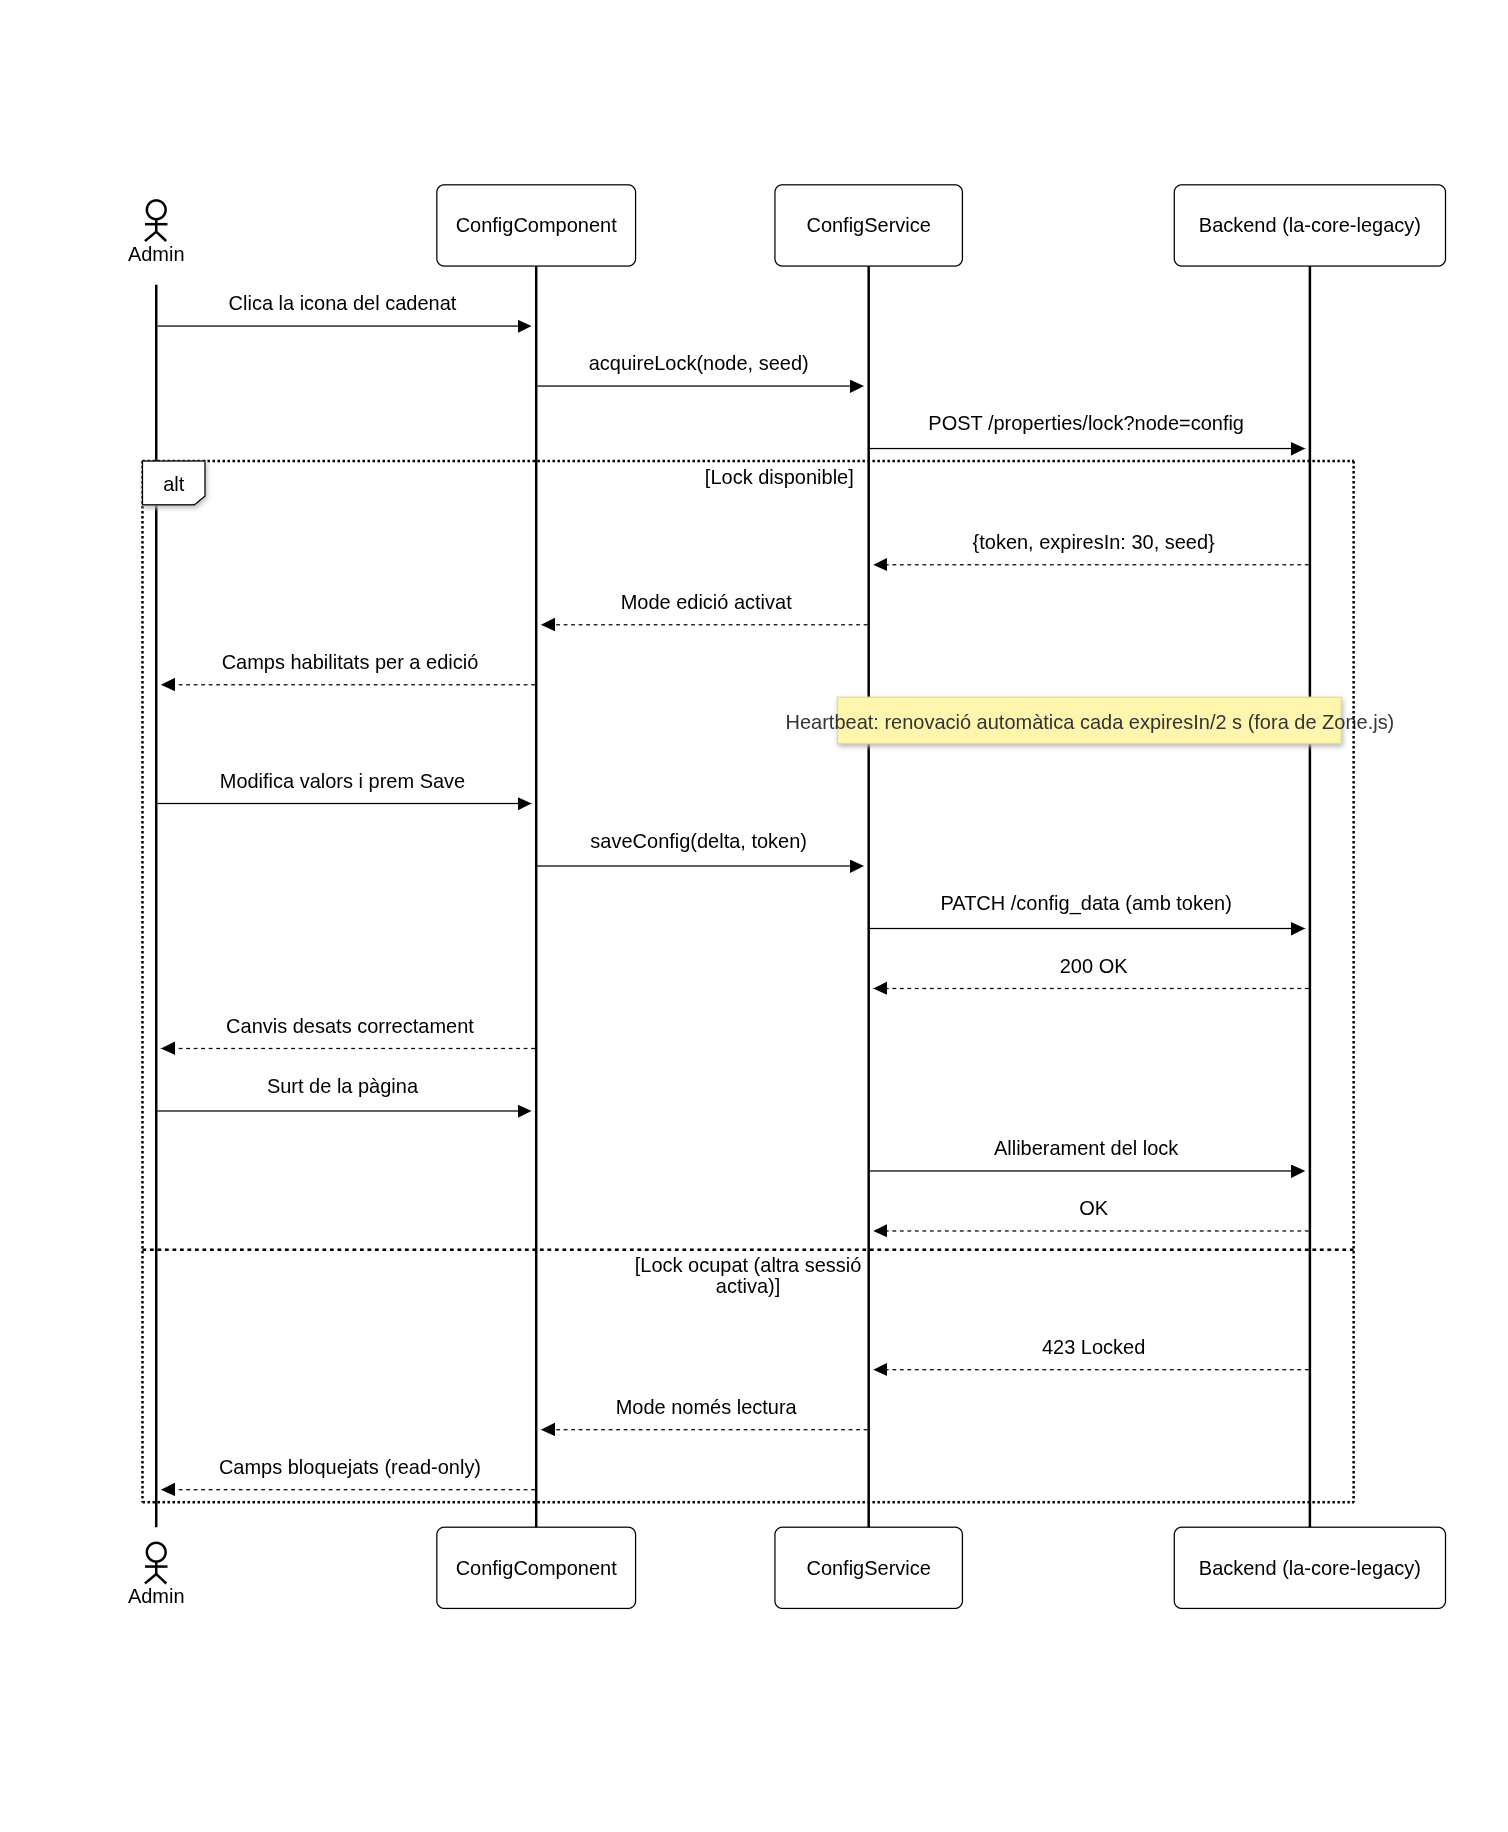
\includegraphics[width=\textwidth,keepaspectratio]{../figures/diagrames/seq_config_lock.png}
      \end{center}
    \end{column}

    \begin{column}{0.50\textwidth}
      \begin{itemize}
        \item \textbf{Adquisició:} POST \texttt{/lock} $\to$ token 32 hex.
        \item \textbf{Expiració:} \textbf{60--120 s} sense renovació.
        \item \textbf{Renovació automàtica:} fora del cicle d'Angular.
        \item \textbf{HTTP 423 Locked} $\to$ mode lectura per a altres.
      \end{itemize}

      \vspace{0.4em}
      \begin{block}{Tolerant a fallades}
        \small Talls de connexió $\Rightarrow$ el cadenat caduca sol. Cap procés queda bloquejat per sempre.
      \end{block}
    \end{column}
  \end{columns}

  \note{
    El disseny del Config Lock va requerir resoldre dos reptes oposats: que el lock fos segur però que no bloquegés indefinidament el sistema en cas de fallada.

    La seguretat es garanteix amb un token de 32 caràcters hexadecimals que cal enviar en cada petició d'escriptura. Si el token no coincideix o ha expirat, el servidor rebutja l'operació.

    La tolerància a fallades es garanteix amb l'expiració automàtica: si l'admin perd la connexió wifi, el torna a tancar el portàtil, o simplement tanca la pestanya sense alliberar el lock, el servidor no queda bloquejat per sempre. El cadenat expira als 60-120 segons i qualsevol altre administrador el pot adquirir.

    La renovació automàtica és transparent per l'usuari i, molt important, no passa pel cicle de detecció d'Angular. Hem implementat una crida HTTP a intervals regulars fora de la Zone.js, de manera que el keep-alive del lock no genera cap re-render innecessari de la interfície.
  }
\end{frame}
